% -*- mode: fundamental -*-

% ****************************************************************

\chapter{RISC-V: the Fife pipelined CPU code}

\markboth{Ch \arabic{chapter}: Fife code}{\copyrightnotice}

\setcounter{page}{1}
% \renewcommand{\thepage}{\arabic{page}}
\renewcommand{\thepage}{\arabic{chapter}-\arabic{page}}

\label{ch_Fife_code}

% ****************************************************************

\section{Introduction}

In this chapter we study BSV code to implement the principles that
were discussed in Chapter~\ref{ch_Fife_Principles}.
We repeat Figure~\ref{Fig_Instr_Exec_w_FIFOs} here, for reference.
\begin{figure}[htbp]
  \centerline{\includegraphics[width=6in,angle=0]{Figures/Fig_Instr_Exec_w_FIFOs}}
  \caption{\label{Fig_Instr_Exec_w_FIFOs_2}Pipelined interpretation of RISC-V instructions (Fig.~\ref{Fig_Instr_Exec} with some annotations)}
\end{figure}

% ****************************************************************

\section{The Fife top-level CPU module}

\label{Sec_Fife_CPU_module}

The code for the top-level Fife CPU module is actually simpler than
the code for the Drum CPU module, because it simply instantiates
sub-modules for each stage and connects them:

\input{Code_Extracts/Fife_mkCPU.tex}

This is practically a direct textual description of
Figure~\ref{Fig_Instr_Exec_w_FIFOs_2}.  The STATE section first
instantiates the pipeline stages shown in the figure.  There is no
explicit module corresponding to Execute Memory Ops---the DMem request
is sent out directly from \verb|stage_RR_RW| and the DMem response is
collected directly by \verb|stage_Retire|.

The STATE section then instantiates the ``forward-flow'' connections
between modules (left to right in the figure), using the
\verb|mkConnection| module to connect a \verb|FIFOF_O| interface
(producer) to a \verb|FIFOF_I| interface (consumer), which was
discussed in Section~\ref{Sec_connecting_FIFOs}.  These module
connections are in the STATE section because, as discussed in
Section~\ref{Sec_connecting_FIFOs} \verb|mkConnection| is just a
module instantiation.

The next few lines instantiate the ``backward-flow'' connections.

In the INTERFACE section, after the \verb|init| method, the next two
lines are the flows of IMem requests from the Fetch stage to memory
and IMem responses from memory to the Decode stage.  These just lift
interfaces from \verb|stage_F| and \verb|stage_D| to the CPU
interface, as is.

The next three lines are for \emph{speculative} DMem access, which we
discussed in Section~\ref{Sec_Store_Buffers}: the flow of DMem
requests from \verb|stage_RR| to memory, the flow of DMem responses
from memory to \verb|stage_Retire|, and the flow of ``commit/discard''
messages from \verb|stage_Retire| to the store-buffer to discharge
STOREs that are waiting in the store-buffer.

The last two lines are for \emph{non-speculative} DMem access, which
we discussed in Section~\ref{Sec_DMem_MMIO}.

Note that the module interface \verb|CPU_IFC| is exactly the same as
in Drum (although Drum has no need for, and does not use the
\verb|DMem_S| speculative interfaces).  Thus, in a system context, we
can directly substitute Drum for Fife and vice versa.  Generalizing
this idea, we can develop other CPUs and substitute them, as well.

We next go through the code for the individual stage modules.

% ****************************************************************

\section{The Fetch stage}

\label{Sec_Fife_Fetch_stage}

The Fetch stage module interface is shown below.  Apart from the
\verb|init| method, the remaining sub-interfaces correspond to the
FIFO-labeled arrows in Figure~\ref{Fig_Instr_Exec_w_FIFOs_2}: the
outgoing \verb|FIFOF_O| interfaces to memory (IMem) and the Decode
stage, and the incoming \verb|FIFOF_I| for redirections from the
Retire stage.

\input{Code_Extracts/Fife_Fetch_IFC.tex}

The Fetch stage module code is shown below.

\input{Code_Extracts/Fife_mkFetch.tex}

The STATE section instantiates various registers and FIFOs.  Next, the
BEHAVIOR section contains two \emph{rules} (Chapter~\ref{ch_Rules_I}).
In rule \verb|rl_Fetch_req|, the explicit condition is the expression:

\hm\small \verb|(rg_running && (! f_F_from_Retire.notEmpty))|

Rule \verb|rl_Fetch_req|'s implicit condition comes from the methods
that it invokes, \verb|f_Fetch_to_Decode.enq ()| and
\verb|f_Fetch_to_IMem.enq ()|.  The rule will fire only when the
explicit condition is true, and when both FIFOs are enabled to enqueue
(have space).  When it fires, it performs the composite action that
comprises all the actions in the rule body:


\begin{itemize}

 \item enqueue the value of \verb|y.to_D| into FIFO \verb|f_Fetch_to_Decode|;

 \item enqueuethe value of \verb|y.mem_req| into FIFO \verb|f_Fetch_to_IMem|;

 \item write the predicted PC value \verb|pred_pc| into register \verb|rg_pc|, and

 \item write the value of \verb|rg_inum+1| into the register \verb|rg_inum|.

\end{itemize}

The right-hand side expressions (\verb|rg_pc+4|, \verb|fn_Fetch(...)| and
\verb|rg_inum+1|) are all combinational circuits, and ``\verb|y|'' is
not a register, just a name for the wires carrying the output value of
\verb|fn_Fetch()|.

% ----------------

\vspace{1ex}

NOTE:
\fbox{\small
\begin{minipage}{5in}

The function {\tt fn\_Fetch()} is exactly the same as the one used in
the Fetch step of Drum (was described in Section~\ref{Sec_fn_Fetch}).

\vspace{1ex}

The types of the messages passed to the Decode stage ({\tt y.to\_D} of
type {\tt F\_to\_D}) and to memory ({\tt y.mem\_req} of type {\tt
Mem\_Req}) are the same as in Drum.

\end{minipage}}

\vspace{1ex}

% ----------------

All these actions are semantically \emph{instantaneous} and
\emph{simultaneous}.  Note that when the rule's implicit and explicit
conditions are true, all the actions are peformed; if false, none of
them are performed, {\ie} the rule is ``atomic''.

In summary, rule \verb|rl_Fetch_req| computes an IMem memory request
from the PC and sends it to memory; it sends auxiliary information to
the Decode stage; and it updates the PC and inum in preparation for
the next Fetch (the next firing of the rule)..

The second rule in the module is \verb|rl_Fetch_from_Retire|. It
receives, in \verb|x|, a redirection message from the Retire stage,
and updates the PC and epoch accordingly.  This rule has no explicit
conditions; its single implicit condition comes from
\verb|f_Fetch_from_Retire|'s implicit condition that we cannot pop a
value from the FIFO until it is non-empty, {\ie}, this rule only fires
when a redirection message is available.  When it fires, it performs
three actions atomically/instantaneously/simultaneously:
 
\begin{itemize}

 \item It dequeues \verb|x| from the FIFO \verb|f_F_from_Retire| (the
       dequeue action is inside the \verb|pop_o| function),
 \item It updates \verb|rg_pc| with the new PC in the redirection message,
 \item It updates \verb|rg_epoch| with the new epoch in the redirection message.

\end{itemize}

Note, \verb|rl_Fetch_from_Retire| updates two registers \verb|rg_pc|
and \verb|rg_epoch| and, \emph{concurrently}, \verb|rl_Fetch| reads
both those registers.  Because rule actions are atomic, we are
guaranteed that \verb|rl_Fetch| will not see inconsitent values in
those two registers, where one has been updated but the other has not
yet been updated.

Finally, the INTERFACE section of the module is simple.  After the
\verb|init| method, we simply lift the FIFO interfaces to the
\verb|mkFetch| module interface.

% ================================================================

\subsection{Prioritizing rule {\tt rl\_Fetch\_from\_Retire} over {\tt rl\_Fetch\_req}}

\index{Rules!prioritizing explicitly}

What would happen if we omit the condition
``\verb|(!f_Fetch_from_Retire.notEmpty)|'' in \verb|rl_Fetch_req|?  It
would not affect the correctness of this module at all.  If we omit
the condition, then both rules could be enabled simultaneously, and it
is non-deterministic which one will fire first.  Actually, the
hardware is deterministic because the \emph{bsc} compiler will make a
prioritization choice, but its choice is unspecified, and so
semantically it is non-deterministic ({\eg} a new release of the
compiler, or a later change in other code in the module may prioritize
differently).  But, for correctness, the choice \emph{does not
matter}.  Because of the atomicity of rules, the rules will never
\emph{interleave} their behavior---either one goes before the other,
or vice versa.  We can quickly reason that, in either case, we get
functionally correct behavior.

The only difference will be in performance: if both rules are enabled,
then, by definition, \verb|rl_Fetch| is fetching ``wrong-path''
instructions due to an earlier misprediction (which is why we have a
redirection).  We know that wrong-path instructions will be discarded
and have no effect.  So if \verb|rl_Fetch| is prioritized, it will
fetch one more wrong-path instruction, with no impact on correctness.

By adding the ``\verb|(!f_Fetch_from_Retire.notEmpty)|'' condition to
\verb|rl_Fetch|, we are explicitly prioritizing
\verb|rl_Fetch_from_Retire| when both are enabled, thus avoiding
\verb|rl_Fetch_req| performing a wasted wrong-path fetch.

% ****************************************************************

\section{The Decode stage}

\label{Sec_Fife_Decode_stage}

The Decode stage module interface is shown below.  Apart from the
\verb|init| method, the remaining sub-interfaces correspond to the
FIFO-labeled arrows in Figure~\ref{Fig_Instr_Exec_w_FIFOs_2}: the
incoming \verb|FIFOF_I| interfaces from the Fetch stage and memory
(IMem), and the outgoing \verb|FIFOF_O| interface to the Register-Read
stage.

\input{Code_Extracts/Fife_Decode_IFC.tex}

The Decode stage module code is shown below.

\input{Code_Extracts/Fife_mkDecode.tex}

The STATE section instantiates FIFOs for incoming and outgoing flows.

The BEHAVIOR section has the single rule \verb|rl_Decode|, whose
implicit conditions will make it wait for both incoming FIFOs
\verb|f_Fetch_to_Decode| and \verb|f_IMem_to_Decode| to be non-empty,
and for its outgoing FIFO \verb|f_Decode_to_RR| to have space.  When
the rule fires, it:

\begin{tightlist}
 \item pops \verb|x| and \verb|rsp_Mem| from the two FIFOs, respectively;

 \item applies function \verb|fn_Decode()| to those values (this is
       the \emph{same} \verb|fn_Decode()| that was used in the Decode
       step of Drum, and described in Section~\ref{Sec_fn_Decode}),
       and

 \item sends the result on to the Register-Read stage.
\end{tightlist}

The INTERFACE section is again straightforward, just lifting the FIFO
interfaces to this module's interface.

% ================================================================

\subsection{Balancing concurrent paths in a pipeline}

\label{Sec_Balancing}

\index{RISC-V!Balancing concurrent paths in a pipeline}

In Figure~\ref{Fig_Instr_Exec_w_FIFOs_2} we see that there are two
concurrent FIFO-like paths from Fetch to Decode: one direct, and the
other via memory (IMem).  Fetch produces two outputs together, one for
each path.  The paths re-converge at Decode, where Fetch's first
output ``meets'' the corresponding response from memory.

\index{RISC-V!In-flight memory transactions}
\index{RISC-V!Memory!pipelined}
\index{RISC-V!Memory!latency}

The path via IMem is also FIFO-like because good memory systems are
themselves pipelined; it is possible for Fetch to issue several
consecutive memory requests before the first response arrives at
Decode.  We say that multiple IMem transactions may be ``in flight''.
Also, in Section~\ref{Sec_mem_latency} we discussed how memory latency
can be variable and unpredictable, so the number of transactions in
flight may vary.

If we wish to allow up to $n$ IMem transactions in flight, then the
direct Fetch-to-Decode path must be capable of buffering up to $n$
\verb|Fetch_to_Decode| items.  If not, rule \verb|rl_Fetch| in Fetch
will get stuck: its \verb|f_Fetch_to_Decode| FIFO will be full, and so
the ``\verb|enq|'' method's implicit condition will become false,
preventing the rule from firing.

This is the reason, in Decode, the incoming \verb|f_Fetch_to_Decode|
FIFO is instantiated with \verb|mkSizedFIFOF(4)|, which is a FIFO with
the capacity to hold four items\footnote{We could also have,
equivalently, instantiated the {\tt f\_Fetch\_to\_Decode} FIFO in
Fetch with {\tt mkSizedFIFO}, or split the buffering capacity between
the two stages.}  We also use the term ``balancing'' for this---the
number of items that can be ``in flight'' in the two paths should be
matched.

Why did we choose the number 4?  Why not something smaller, or larger?
Greater capacity requires more hardware resources, which argues for a
smaller number, but a smaller number may affect performance where
Fetch has to wait only because of limited capacity.  We would like to
choose the smallest number that covers the number of IMem transactions
that may be in flight (memory latency, or depth of IMem pipeline).
But that number varies with memory system design and, even for a
particular design, it varies over time---it depends on the particular
RISC-V program running, the memory system's caches, hits and misses,
cache interactions, cache miss latencies, and so on\footnote{With
virtual memory, it will also depend on TLB misses and the latency of
page table walks.}  Thus, there is no obvious ``optimal'' choice for
\verb|mkSizedFIFOF| capacity; we must ``tune'' the number by running
the CPU on desired applications, with different FIFO capacities,
observe the effect on performance and resources, and pick an
``acceptable'' capacity.

% ****************************************************************

\section{The Register-Read and Dispatch (and Register-Write) stage}

\label{Sec_Fife_RR_RW_stage}

The Register-Read and Dispatch module contains (instantiates) the GPRs
register file (Section~\ref{Sec_RISCV_regfile}) and the scoreboard to
manage read-write hazards (Section~\ref{Sec_Scoreboards}).  In the
forward flow,

\begin{itemize}

  \item it stalls (waits) if the instruction has rs1, rs2 or rd, and
        these are busy according to the scoreboard;

  \item it reads rs1 and rs2 registers for the current instruction;

  \item it sets the scoreboard for the current instruction's rd to 1,
        marking it ``busy'' (if the instruction has an rd);

  \item it uses information from the Decode stage to dispatch to the
        four Execute pipes.  We always (for every instruction) send an
        execution tag and additional information on the direct path to
        Retire.  Depending on the instruction, it may also send
        information into one of the other Execute pipes:

  \begin{tightlist}
    \item Execute Control
    \item Execute Integer
    \item memory (a DMem request)
  \end{tightlist}

\end{itemize}

This stage also participates in a backward flow, because the GPRs
register file and scoreboard are instantiated here.  When an
instruction is completed, the Retire stage sends a message to this
module to update those components: release an rd reservation in the
scoreboard and write-back an rd register value.

The interface for the Register-Read and Dispatch stage module is shown
below.  Apart from the \verb|init| method, the remaining
sub-interfaces correspond to the FIFO-labeled arrows in
Figure~\ref{Fig_Instr_Exec_w_FIFOs_2}: the incoming \verb|FIFOF_I|
interface from the Decode stage, the outgoing \verb|FIFOF_O|
interfaces direct to Retire and to Execute Control, Execute Int and to
DMem, and an incoming \verb|FIFOF_I| from Retire for updating the
register file and scoreboard, which are instantiated inside this
module.

\input{Code_Extracts/Fife_RR_RW_IFC.tex}

% ================================================================

\subsection{BSV: Vectors for the Scoreboard}

\label{Sec_Fife_Scoreboard}

\index{BSV!vector@{\tt vector}!library data type}

In Section~\ref{Sec_Scoreboards} we discussed the general principles
of a scoreboard, and described it as an array of 1-bit values.  In BSV
the following type is used to represent an array of $n$ items, each of
which is of type $t$:

\begin{tabbing}\small\tt
\hmm Vector \#(n, t);
\end{tabbing}

Note: in order to use this type in any BSV code file, the file must
import the \verb|Vector| library:

\begin{tabbing}\small\tt
\hmm import Vector :: *;
\end{tabbing}

So, we can define a \verb|Scoreboard| type as follows:
\begin{tabbing}\small\tt
\hmm typedef  Vector \#(32, Bit \#(1))  Scoreboard;
\end{tabbing}

\index{BSV!replicate@{\tt replicate} {\tt vector} library function to create a vector value}
\index{BSV!vector@{\tt vector}!library {\tt replicate} function}

The BSV Vector-library function:

\begin{tabbing}\small\tt
\hmm replicate (v)
\end{tabbing}

creates a value of type \verb|Vector #(n, t)| where $n$ is inferred
from the context and \verb|v| has the type $t$.  All $n$ items in the
value are equal to \verb|v|.  Thus, we can instantiate a scoreboard
like this, where all the vector elements are initialized to 0:

\begin{tabbing}\small\tt
\hmm Reg \#(Scoreboard) rg\_scoreboard <- mkReg (replicate (0));
\end{tabbing}

\index{BSV!vector@{\tt vector}!of {\tt n} bits \emph{vs.} {\tt Bit\#(n)}}
\index{BSV!vector@{\tt vector}!representation in bits}

In hardware, a \verb|Vector#(32,Bit#(1))| value occupies exactly 32
bits, {\ie} the size of the vector times the size of each element.
So, why not use \verb|Bit #(32)| instead?  It's a matter of
programming taste:

\begin{tightlist}

  \item The same syntax \verb|v[j]| works both for bit-selection from
        \verb|Bit#(n)| and \verb|Vector#(n,Bit#(1))|.

  \item With \verb|Bit#(n)|, a $j^{th}$ bit can also be selected using
        shift-and-mask operations: \verb|((v >> j) & 1)|.

  \item The $j^{th}$ bit of \verb|Vector#(n,Bit#(1))| can be updated
        using simple assignment \\
	\hmm \verb|v [j] = new_value;|

  \item The $j^{th}$ bit of \verb|Bit#(n)| can be updated using shift
        and mask operations: \\
	\hmm \verb'(v | (1 << j))' to set the $j^{th}$ bit to 1, and \\
	\hmm \verb|(v & (~ (1 << j)))| to resset the $j^{th}$ bit to 0

\end{tightlist}

We can convert a \verb|Vector #(32, Bit #(1))| value into a \verb|Bit#(32)| value with:

\hmm \verb|pack (v)|

and we can convert a \verb|Bit#(32)| value into a \verb|Vector #(32, Bit #(1))| value with:

\hmm \verb|unpack (v)|

% ================================================================

\subsection{The Register-Read and Dispatch (and Register-Write) module}

\label{Sec_mkRR_RW}

The first part of the \verb|mkRR_RW| module, instantiating its STATE, is shown below:

\input{Code_Extracts/Fife_mkRR_RW1.tex}

It instantiates FIFOs for all the forward and backward flows, and it
instantiates the GPRs register file \verb|gprs|
(Section~\ref{Sec_RISCV_regfile}) and the \verb|scoreboard|
(Section~\ref{Sec_Scoreboards}).  The second part of the
\verb|mkRR_RW| module, implementing its BEHAVIOR for the forward flow,
is shown below:

\input{Code_Extracts/Fife_mkRR_RW2.tex}

In line 6, we observe the first element in the \verb|f_Decode_to_RR|
FIFO.  Note, the \verb|.first| method is non-destructive, {\ie} it
merely observes and \emph{does not dequeue} the first element from the
FIFO.  This is because, if we must stall, it needs to be available
again the next time the rule fires.

The next several lines compute the stall condition by checking the
scoreboard for whether rs1, rs2 or rd are busy (if the instruction has
rs1, rs2 or rd, respectively).

If we stall, the rule takes no action; everything will be retried the
next time it fires.

If we do not stall, then we dequeue the \verb|f_Decode_to_RR| FIFO.
We read values of the rs1 and rs2 registers.  Note, if the instruction
does not have an rs1 or rs2, here we will be reading some random
registers according to the bits that happen to be in the rs1 and rs2
bit-positions in the instruction.  This does not matter; in the
Execute stage each instruction only \emph{uses} these values if the
instruction has an rs1 and/or rs2.

Next, we apply the function \verb|fn_Dispatch()| (discussed in
Section~\ref{Sec_fn_Dispatch}, and is the same one we use in Drum) to
the inputs, which computes \verb|y|, containing the structs to be sent
on the direct path (\verb|y.to_Retire|), to Execute Control
(\verb|y.to_Control|), and to Execute Int and Execute DMem
(\verb|y.toEX|).

If the instruction has an rd, we mark it on the scoreboard.  We
enqueue \verb|y.to_Retire| on the direct flow (FIFO
\verb|f_RR_to_Retire|).

The remaining code is a nested if-then-else that sends information
into the appropriate Execute pipe (Execute Control, Execute Integer,
or DMem).

% ----------------
\hdivider

\Exercise

Consider this hypothetical scenario: suppose the \verb|stall|
condition is false.  Then, we need to dequeue \verb|f_Decode_to_RR|
and do one or more enqueues into \verb|f_RR_to_Retire| and
\verb|f_RR_to_EX_Control|, \verb|f_RR_to_EX_Int| or
\verb|f_DMem_S_req.enq|.  Is it possible that we perform the dequeue
and then are unable to perform the enqueue(s) because the
corresponding output FIFO happens to be full?

\emph{Hint:} rule atomicity

\Exercise

Write a boolean expression representing the overall firing condition
for the rule.  Briefly: all FIFO-modifying actions (dequeue, enqueue)
have implicit conditions, but for each FIFO, that condition is only
relevant if the conditions on the surrounding if-then-else's select
that action.

% ----------------
\hdivider

\Exercise

When debugging the implementation, it is useful to know if, due to
some coding mistake, rule \verb|rl_RR_Dispatch| is stalled forever.
For example, for some instruction with an rd, if the Retire stage did
not send back the rd's scoreboard-release, that register will be
forever ``busy''.

Add a register to count consecutive stalls, initially 0.  In the rule,
whenever we successfully dispatch an instruction, reset the counter to
0.  Whenever we stall, increment the stall counter, and if the
stall-counter reaches some chosen threshold value, prints debugging
messages and executes \verb|$finish| to terminate simulation.

\Endexercise
% ----------------

The third part of the \verb|mkRR_RW| module, implementing its BEHAVIOR
for the backward flow, is shown below:

\input{Code_Extracts/Fife_mkRR_RW3.tex}

We pop the message \verb|x| from the \verb|f_RW_from_Retire| FIFO.  We
perform its specified scoreboard-release for register rd.  If the rd
value is to be committed, we write it into GPR [rd].  The fourth and
final part of the \verb|mkRR_RW| module, defining its INTERFACE, is
shown below:

\input{Code_Extracts/Fife_mkRR_RW4.tex}

It simply lifts the FIFO interfaces to this module's interface.

% ****************************************************************

\section{The Execute Control stage}

\label{Sec_Fife_Control_stage}

The interface for the Execute Control stage module is shown below.
Apart from the \verb|init| method, the remaining sub-interfaces
correspond to the FIFO-labeled arrows in
Figure~\ref{Fig_Instr_Exec_w_FIFOs_2}: the incoming \verb|FIFOF_I|
interface from the Register-Read and Dispatch stage and the outgoing
\verb|FIFOF_O| interface to the Retire stage.

\input{Code_Extracts/Fife_EX_Control_IFC.tex}

The Execute Control stage module is shown below:

\input{Code_Extracts/Fife_mkEX_Control.tex}

After instantiating the forward flow input and output FIFOs, the rule
\verb|rl_EX_Control| simply applies the function \verb|fn_Control| to
each input and enqueues the output.  This function was described in
Section~\ref{Sec_fn_EX_Control}, and is the same one we use in Drum.
Finally, the interface, after the \verb|init| method, simply lifts the
FIFO interfaces to the interface of this module.

% ****************************************************************

\section{The Execute Integer Ops stage}

\label{Sec_Fife_EX_Int_stage}

The interface for the Execute Integer stage module is shown below.
Apart from the \verb|init| method, the remaining sub-interfaces
correspond to the FIFO-labeled arrows in
Figure~\ref{Fig_Instr_Exec_w_FIFOs_2}: the incoming \verb|FIFOF_I|
interface from the Register-Read and Dispatch stage and the outgoing
\verb|FIFOF_O| interface to the Retire stage.

\input{Code_Extracts/Fife_EX_Int_IFC.tex}

The Execute Integer stage module is shown below:

\input{Code_Extracts/Fife_mkEX_Int.tex}

After instantiating the forward flow input and output FIFOs, the rule
\verb|rl_EX_Int| simply applies the function \verb|fn_EX_Int| to each
input and enqueues the output.  This function was described in
Section~\ref{Sec_fn_EX_Int}, and is the same one we use in Drum.
Finally, the interface, after the \verb|init| method, simply lifts the
FIFO interfaces to the interface of this module.

% ****************************************************************

\section{The Execute Memory Ops stage (speculative DMem)}

\label{Sec_Fife_DMem_stage}

There is no explicit code for an Execute Memory Ops stage.  The
forward-path rule \verb|rl_RR_Dispatch| in the
Register-Read-and-Dispatch stage, described in
Section~\ref{Sec_Fife_RR_RW_stage}, directly enqueues a memory request
that goes out to memory.  The Retire stage, to be discussed in
Section~\ref{Sec_Fife_Retire_code}, consumes the corresponding memory
response.

% ****************************************************************

\section{Fife: the Retire stage}

\label{Sec_Fife_Retire_code}

This module is longer than the others only because it takes care of
many possible cases as outlined in Figure~\ref{Fig_Fife_Retire_2}
(which repeats Figure~\ref{Fig_Fife_Retire} here for reference).
\begin{figure}[htbp]
  \centerline{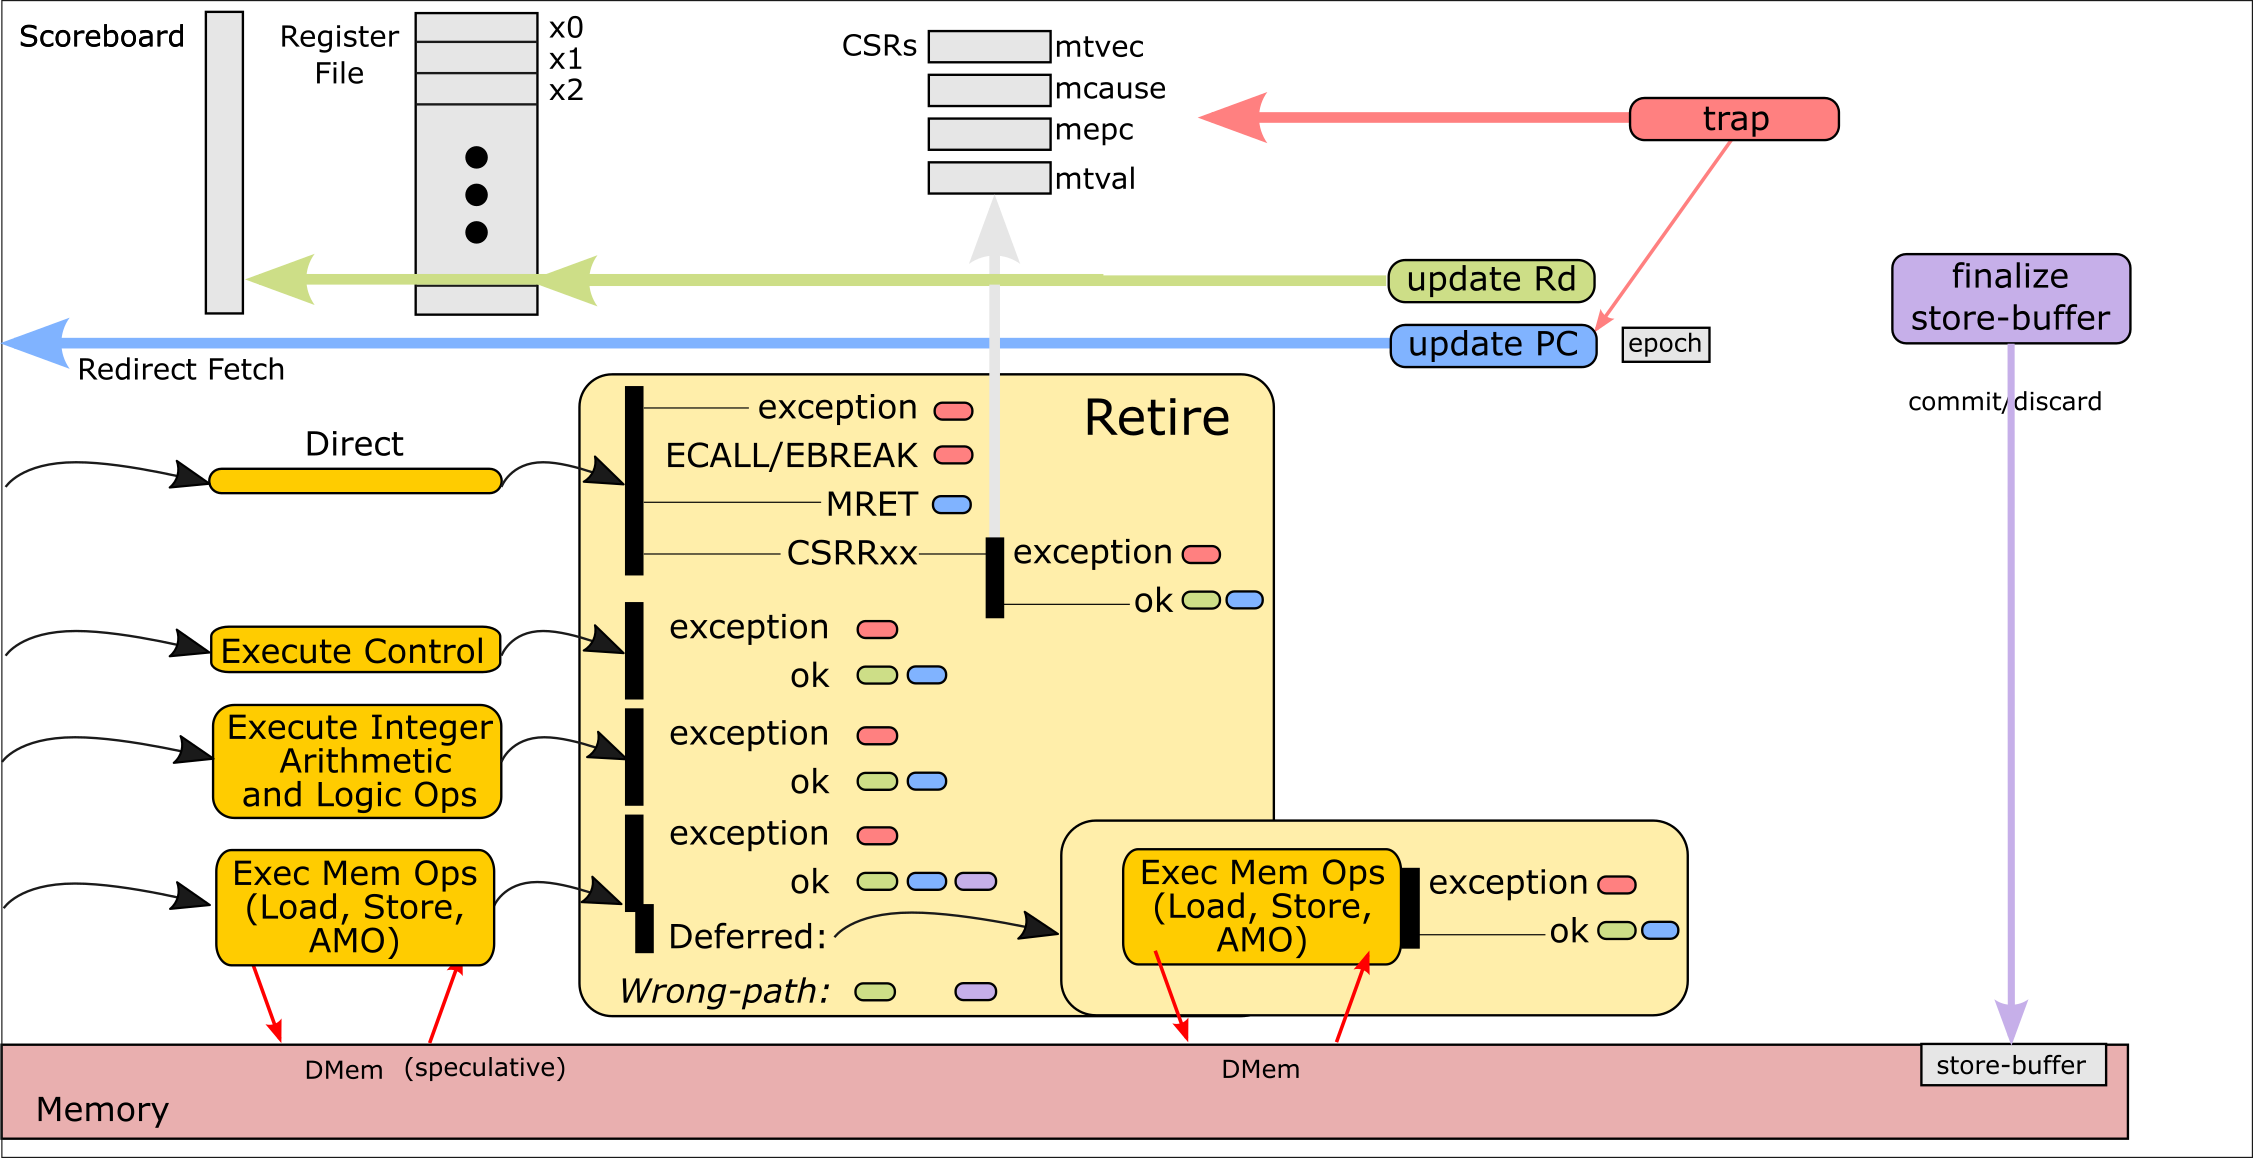
\includegraphics[width=6in,angle=0]{Figures/Fig_Retire_Layers_1_2}}
  \caption{\label{Fig_Fife_Retire_2}
           Actions in the ``Retire'' stage of Fife
	   (same as Fig.~\ref{Fig_Fife_Retire})}
\end{figure}

Here is the interface definition for this module:

\input{Code_Extracts/Fife_Retire_IFC.tex}

The first four \verb|FIFO_I| sub-interfaces correspond to the black
arrows entering the Retire module from the execute pipes (left of
Retire module in the figure).

The next \verb|FIFO_O| interface, \verb|fo_DMem_S_commit|, is the
purple arrow sending commit/discard messages to the store-buffer.

The next two sub-interfaces are red arrows connecting the second Exec
Mem Ops box to memory (non-speculative DMem request and response).

The last two \verb|FIFO_O| sub-interfaces are the blue arrow at the
top of the figure carrying redirections to the Fetch stage, and the
green arrow carrying Register-Writes to the \verb|RR_RW| module.

This module has a mixture of modes.  Normally it is in pipeline mode,
receiving instructions from the Execute stages and retiring them.  In
certain circumstances, it goes into FSM mode, similar to Drum:

\begin{tightlist}

 \item Execute non-speculative DMem ops (MMIO/non-memory-like),
        FSM-sequencing through issuing a request to memory and
        handling the response.

 \item Execute a CSRRxx insruction, which may raise an exception,
       which must then be handled.

 \item Execute traps (for exceptions or interrrupts).

\end{tightlist}

We define a ``module mode'' to reflect these modes:

\input{Code_Extracts/Fife_Retire_Module_Mode.tex}

The first part of the Retire stage \verb|mkRetire| module is shown below.

\input{Code_Extracts/Fife_mkRetire1.tex}

It instantiates the CSR registers (Section~\ref{Sec_RISCV_CSRs}), and
register \verb|rg_epoch| to keep track of the epoch
(Section~\ref{Sec_Epochs}), and then FIFOs for all the incoming and
outgoing channels.  Finally, it instantiates register \verb|rg_mode|
to hold the current module mode, and a couple of registers to hold
exception information until we can perform the exception actions.

% ================================================================

\subsection{Common facilities used by many rules}

\label{Sec_Retire_Common}

Before we study the rules in the module, we first encapsulate, in
\verb|Action| functions, some common actions performed in many rules.

The following function captures the actions to be taken whenever we
need to redirect the Fetch stage to start fetching from a different
PC.  This can be due to a misprediction of the successor of the
current instruction, or due to an exception or MRET.

\input{Code_Extracts/Fife_fa_redirect_Fetch.tex}

The boolean \verb|mispredicted| indicates whether the prediction was
correct or not.  If the prediction was correct, no action is taken.
Otherwise, we increment \verb|rg_epoch|, and send a redirection
message to the Fetch stage with the correct PC and the new epoch.  The
consumption of this message in the Fetch stage was discussed in
Section~\ref{Sec_Fife_Fetch_stage}.

The following function captures the actions to be taken for updating
an instruction's destination rd register. If the instruction has an rd
register, it assembles a \verb|RW_to_Retire| message and sends it to
the \verb|RR_RW| module.  The consumption of this message in the
Register-Read and Dispath (and Register-Write) stage was discussed in
Section~\ref{Sec_Fife_RR_RW_stage}.

\input{Code_Extracts/Fife_fa_update_rd.tex}

The following function sends a commit/discard message to the
speculative DMem store-buffer, if the instruction writes to memory:

\input{Code_Extracts/Fife_fa_retire_store_buf.tex}

The \verb|f_RR_to_Retire| (direct path) FIFO contains an entry for
\emph{every} instruction.  Information in the first element tells us
how to retire it, including which of the execute pipes need to be
examined.  The following definitions capture some properties of this
first element.

\input{Code_Extracts/Fife_triage.tex}

The incoming instruction is a wrong-path instruction if its
accompanying epoch does not match our \verb|rg_epoch| register.

% ================================================================

\subsection{Rule to retire wrong-path instructions (all paths; discard)}

For a wrong-path instruction, we dequeue it from \verb|f_RR_to_Retire|.

If it has an Rd, we send a discard-scoreboard-reservation message to
the RR-RW module using \verb|fa_update_rd()|.

If it was a Control, Int or DMem instruction, we dequeue it from the
corresponding incoming FIFO.  In the DMem case, if it did a
speculative STORE, we also send a ``discard'' message to the head of
the store-buffer using \verb|fa_retire_store_buf()|.

\input{Code_Extracts/Fife_rl_wrong_path.tex}

% ================================================================

\subsection{Rules to retire from direct path}

The following subsections handle instruction-retirement for the cases
where the direct-path has all the necessary information, i.e., where
the instruction was not dispatched into the Execute Control, Execute
Int or Execute DMem paths.

% ----------------------------------------------------------------

\subsubsection{Rule to retire CSRRxx instructions (direct path)}

\label{Sec_Fife_Retire_CSRRxx}

The following rule handles CSRRxx instructions, which arrive on the direct path:

\input{Code_Extracts/Fife_rl_CSRRxx.tex}

The rule's explicit condition restricts it to fire only when we are in
PIPE mode and when the next instruction is not a wrong-path
instruction (epoch is correct), is a Direct-path instruction, is not
an exception, and is indeed a CSRRxx instruction.

If so, it applies \verb|csrs.csrrxx()| (described in
Section~\ref{Sec_RISCV_CSRs}, and the same one we used in Drum), and
updates the rd register with the result.

If the CSRRxx operation did not raise an exception, it redirects Fetch
this instruction's successor was mispredicted.

If the CSRRxx operation raised an exception, we save the details in
some registers and switch from PIPE mode into EXCEPTION mode; this
will enable rule \verb|rl_exception|
(Section~\ref{Sec_Fife_Exception}) to handle it.

Why postpone exception-handling to the later rule?  Why not perform
that rule's action here?  The reason is to avoid contention on the CSR
registers.  Rule \verb|rl_Retire_CSRRxx| invokes method
\verb|csrs.mav_csrrrxx()| and rule \verb|rl_exception| invokes method
\verb|csrs.mav_exception()|.  By separating these invocations into two
separate rules, we avoid contention between these two CSR module
methods.

% ----------------

\Exercise

The provided implementation of the CSR registers
(Section~\ref{Sec_RISCV_CSRs}) will in fact prevent the two methods
\verb|csrs.mav_csrrrxx()| and \verb|csrs.mav_exception()| from being
invoked in a single action, {\ie} in a single rule, due to
method-ordering constraints.  Try this experiment: copy the body of
\verb|rl_exception| into \verb|rl_Retire_CSRRxx|; try compiling it
with \verb|bsc|, and observe the compiler's complaint message.

\Exercise

Modify the CSRs module method \verb|mav_csrrxx()| to combine the
actions of the original \verb|mav_csrrrxx()| with the actions of
\verb|mav_exception()|.  The result type will have to be extended
(say, a 3-tuple) to also return the trap-vector PC in case of an
exception.  Modify \verb|rl_Retire_CSRRxx| so that it immediately does
a Fetch-redirect with the trap-vector PC in case of an exception.
There is no longer any need to shift out of \verb|MODE_PIPE| into
\verb|MODE_EXCEPTION|.

\vspace{1ex}

This will save a cycle in handling CSRRxx instructions.  But what is
the impact on hardware complexity in the \verb|mkCSRs| module?

\Endexercise
% ----------------

% ----------------------------------------------------------------

\subsubsection{Rules to retire MRET instructions (direct path)}

The following rule handles MRET instructions, which arrive on the direct path:

\input{Code_Extracts/Fife_rl_MRET.tex}

Again, pay careful attention to the rule's explicit condition which
restricts it to fire only when we are in PIPE mode and when the next
instruction is not a wrong-path instruction (epoch is correct), is a
Direct-path instruction, is not an exception, and is indeed an MRET
instruction.

The rule body is simple---always redirect to the PC found in the CSR
MEPC (Section~\ref{Sec_Traps}).

% ----------------------------------------------------------------

\subsubsection{Rules to retire ECALL and EBREAK instructions (direct path)}

The following rule handles ECALL and EBREAK instructions, which arrive on the direct path:

\input{Code_Extracts/Fife_rl_ECALL.tex}

The rule's explicit condition restricts it to fire only when we are in
PIPE mode and when the next instruction is not a wrong-path
instruction (epoch is correct), is a Direct-path instruction, is not
an exception, and is indeed an ECALL or EBREAK instruction.

ECALL and EBREAK are just deliberately-invoked exceptions, the only
difference being the exception-code we pass in the \verb|mcause| CSR
(Section~\ref{Sec_ECALL_EBREAK}).  We save appropriate exception
values and switch from \verb|MODE_PIPE| to \verb|MODE_EXCEPTION|,
which will handle the exception.

% ----------------

\Exercise

In the exercises in Section~\ref{Sec_Fife_Retire_CSRRxx}, we discussed
why, in \verb|rl_Retire_CSRRxx| we postponed exception handling to the
separate rule \verb|rl_exception|: \verb|rl_Retire_CSRRxx| itself
accesses the CSRs, and \verb|rl_exception| accesses the CSRs, and we
wanted to avoid contention.

\vspace{1ex}

Here, \verb|rl_Retire_ECALL_EBREAK| does not otherwise access the
CSRs, so there is no such contention, so why not handle the exception
directly here (copy the body of \verb|rl_exception| here) and save a
cycle?  Discuss the impact on hardware structure.  Try it, examine the
generated Verilog, and examine the performance impact (which will
depend on the RISC-V program being run, of course).

\Endexercise
% ----------------

% ----------------------------------------------------------------

\subsubsection{Rules to retire exceptions from the direct path}

The following rule handles exceptions which arrive on the direct path:

\input{Code_Extracts/Fife_rl_Dir_Exc.tex}

The rule's explicit condition restricts it to fire only when we are in
PIPE mode and when the next instruction is not a wrong-path
instruction (epoch is correct), is a Direct-path instruction, and is
an exception.

The rule does nothing more than save the exception information in
registers and move from \verb|MODE_PIPE| to \verb|MODE_EXCEPTION| so
that the exception will be handled by \verb|rl_exception|.

% ================================================================

\subsection{Rules to retire from the Execute Control path}

\label{Sec_Fife_Retire_Control}

The following rule handles instructions (BRANCH, JAL, JALR) that
arrive on the Execute Control path.  In Execute Control, it could have
succeeded or it could have raised an exception (if the
control-transfer target PC was misaligned).

\input{Code_Extracts/Fife_S5_Control.tex}

We dequeue the direct-path information (\verb|f_RR_to_Retire|) and we
pop the Execute Control path information
(\verb|f_EX_Control_to_Retire|).

We invoke \verb|fa_update_rd()| to update the destination register
(JAL and JALR may save a ``return address'' in rd) and its scoreboard
reservation.  Recall from Section~\ref{Sec_Retire_Common} that
\verb|fa_update_rd()| will not send any update message if the
instruction does not have an rd (or if rd is 0).  The
``\verb|(!x2.exception)|'' argument to \verb|fa_update_rd()| ensures
that if there was an exception only the scoreboard reservation will be
released, and no register value will be written.

If there was no Execute Control exception, we redirect the Fetch stage
if mispredicted.  At this point we know both what was predicted as the
successor PC and what is the actual successor PC for this instruction,
so we can compare these to determine if there was a misprediction.

If there was a Execute Control exception, we save relevant values in
registers and move from \verb|MODE_PIPE| to \verb|MODE_EXCEPTION|
which will enable \verb|rl_exception| to perform the required actions.

% ================================================================

\subsection{Rules to retire from the Execute Integer path}

\label{Sec_Fife_Retire_Int}

The following rule handles LUI, AUIPC and Integer instructions that
arrive on the Execute Integer path.  Note, none of these standard
RISC-V instructions raise any exceptions.  However, in this rule we
assume the possibility of an instruciton in case, in future, we extend
Fife's supported ISA with new non-standard Integer instructions that
could raise an exception.

\input{Code_Extracts/Fife_S5_Int.tex}

We dequeue the direct-path information (\verb|f_RR_to_Retire|) and we
pop the Execute Int path information (\verb|f_EX_Int_to_Retire|).

We invoke \verb|fa_update_rd()| to update the destination register and
its scoreboard reservation.  Recall from
Section~\ref{Sec_Retire_Common} that \verb|fa_update_rd()| will not
send any update message if the instruction does not have an rd (or if
rd is 0).  The ``\verb|(!x2.exception)|'' argument to
\verb|fa_update_rd()| ensures that if there was an exception only the
scoreboard reservation will be released, and no register value will be
written.

If there was no Execute Integer exception, we redirect the Fetch stage
if mispredicted.  We can compare the predicted successor PC for this
instruction with its fall-through PC to determine if there was a
misprediction.

If there was an Execute Integer exception, we save relevant values in
registers and move from \verb|MODE_PIPE| to \verb|MODE_EXCEPTION|
which will enable \verb|rl_exception| to perform the required actions.

% ================================================================

\subsection{Rules to retire from the Execute DMem path, or perform deferred DMem request}

\label{Sec_Fife_S5_DMem}

The following rules handle instructions that arrive on the Execute
DMem path.  This path could have raised an exception (bad address,
misaligned, memory-permission violation).  Or, it could have performed
a speculative LOAD/STORE/AMO successfully, but if it wrote to memory,
the value is still sitting in the store-buffer and needs to be
committed.  Or, it could have been deferred because the memory address
was a non-memory-like location ({\eg} MMIO) that did not allow
speculation.  The first two cases are handled by the first rule below;
the deferred case is handled by rules described subsequently.

% ----------------------------------------------------------------

\subsubsection{Retire speculative and exception from DMem}

\label{Sec_Fife_Retire_DMem}

The following rule handles incoming DMem exceptions and successful
speculative results.

\input{Code_Extracts/Fife_S5_DMem.tex}

Note that the rule condition excludes deferred requests (they are
handled in another rule, described in the next section).

We dequeue the direct-path information (\verb|f_RR_to_Retire|) and we
pop the Execute DMem path information (\verb|f_EX_DMem_S_Rsp|).

We invoke \verb|fa_update_rd()| to update the destination register and
its scoreboard reservation.  Recall from
Section~\ref{Sec_Retire_Common} that \verb|fa_update_rd()| will not
send any update message if the instruction does not have an rd (or if
rd is 0).  The ``\verb|(!x2.exception)|'' argument to
\verb|fa_update_rd()| ensures that if there was an exception only the
scoreboard reservation will be released, and no register value will be
written.

If there was no Execute Dmem exception, we send a ``commit'' message
to the store buffer and redirect the Fetch stage if mispredicted.  We
can compare the predicted successor PC for this instruction with its
fall-through PC to determine if there was a misprediction.  Note that
``\verb|fa_retire_store_buf()|'' will send a commit message only if
the instruction wrote memory (Section~\ref{Sec_Retire_Common}).

If there was an Execute DMem exception, we save relevant values in
registers and move from \verb|MODE_PIPE| to \verb|MODE_EXCEPTION|
which will enable \verb|rl_exception| to perform the required actions.
The RISC-V ``cause code'' is computed based on the kind of DMem
exception and the kind of instruction.

% ----------------

\Exercise

Inside \verb|rl_Retire_EX_DMem| we invoke ``\verb|fa_update_rd()|''
always, but we invoke ``\verb|f_retire_store_buf()|'' only when there
was no exception.  Justify this.

\Endexercise
% ----------------

% ----------------------------------------------------------------

\subsubsection{Rule handle deferred DMem requests (from Execute DMem path)}

\label{Sec_Fife_DMem_deferred}

The following rule handles memory requests that were deferred by the
Execute DMem stage because there could not be performed speculatively.

\input{Code_Extracts/Fife_S5_Deferred.tex}

We pop the Execute DMem result (\verb|f_DMem_S_rsp|).  We do not
dequeue the direct-path (\verb|f_RR_to_Retire|) because we will need
that informnation when we later handle the DMem response; we leave it
at the head of the FIFO.

We merely construct the memory request now, and send it to memory
(enqueue it on \verb|f_DMem_req|).  We also switch out of
\verb|MODE_PIPE| into \verb|MODE_DMEM_RSP| which enables rule
\verb|rl_Retire_DMem_rsp| (described next) to await the memory
response.

% ----------------------------------------------------------------

\subsubsection{Rules to retire responses for deferred DMem requests}

\label{Sec_Fife_Retire_DMem_deferred}

The following rule handles the corresponding responses from memory.

\input{Code_Extracts/Fife_S5_Deferred_rsp.tex}

We can now dequeue the direct-path information (\verb|f_RR_to_Retire|)
and the memory-response (\verb|f_DMem_Rsp|).

If the response returned an exception, we compute the RISC-V exception
\verb|cause| code, save values in registers, and move to
\verb|MODE_EXCEPTION| so that \verb|rl_exception| can handle it
subsequently.

The memory system should \emph{never} return a \verb|MEM_REQ_DEFERRED|
for these requests through the non-speculative memory interface;
responses can only be OK or an exception.  The middle
``\verb|else-if|'' clause is just a bit of defensive programming in
case of a buggy memory system.

If the response was OK, we invoke \verb|fa_update_rd()| to update the
destination register and its scoreboard reservation.  Recall from
Section~\ref{Sec_Retire_Common} that \verb|fa_update_rd()| will not
send any update message if the instruction does not have an rd (or if
rd is 0).  The second argument is True because this not the exception
case.

Finally, we redirect the Fetch stage if mispredicted, and return to
\verb|MODE_PIPE| to resume pipeline processing.  We can compare the
predicted successor PC for this instruction with its fall-through PC
to determine if there was a misprediction.

% ----------------

\Exercise

This rule fields a memory response, but does not send any
commit/discard message to the store-buffer.  Why not?

\Endexercise
% ----------------

% ================================================================

\subsection{Common Rule to handle exceptions}

\label{Sec_Fife_Exception}

This is a common rule used to handle exceptions.

\input{Code_Extracts/Fife_S5_exc.tex}

In all the previous rules, when an exception is detected, we save
relevant values in registers \verb|rg_epc|, \verb|rg_cause| and
\verb|rg_tval| and switch the module mode to \verb|MODE_EXCEPTION|,
which enables this rule.  It invokes \verb|csrs.mav_exception()| which
updates the relevant CSRs, and returns the value CSR \verb|mtvec|
(trap-vector PC).  Here, we simply redirect to that PC, and return to
pipeline processing in \verb|MODE_PIPE|.

% ================================================================

\subsection{Fife module interface definition}

The final INTERFACE section, as with other modules, has an \verb|init|
method, and then lifts the various FIFO interfaces into sub-interfaces
for this module.

\input{Code_Extracts/Fife_mkRetire_ifc.tex}

% ****************************************************************

\section{Conclusion}

And that is the complete Fife CPU!  There is actually very little in
this chapter that is RISC-V specific; these pipeline structures are
needed for a pipelined CPU for \emph{any} ISA.  All our
RISC-V-specific discussions were completed in the chapters leading up
to Drum, and here we have simply reused all those RISC-V-specific
common functions.

There is quite a lot scope for performance optimization here, even
keeping the same pipeline structure.  For example:

\begin{itemize}

\item The sooner we can deliver a redirection from Retire to Fetch,
      the less time the CPU will waste fetching and discarding
      wrong-path instructions.

\item In a message from Retire to the Register-Read and Dispatch stage
      to update rd and release the scoreboard, the sooner we can
      deliver that value to any waiting instruction, the less time
      wasted in waiting on the scoreboard.

\item In Retire, the \verb|rl_exception| actions can be folded in to
      the rule where the exception is detected, avoiding another
      delay, except possibly in the CSRRxx case, where there may be
      contention with CSR access.

\end{itemize}

We will discuss how to do some of these optimizations in
Chapter~\ref{ch_Rules_II}.

It is not straightforward to judge whether an optimization is worth it
or not.  Many optimizations add hardware cost (silicon area and energy
consumption).  Some optizationw, while reducing the number of clocks
for a computation, may require slower clock speeds because of longer
combinational paths, thus negating some of the speed advantage.

Because of the high variability in the mix of instructions across
different programs, some optimizations may have more effect on some
programs than on others.

Ultimately, the value of most optimizations cannot be judged in the
abstract, only in specific contexts: What are the actual application
programs that will be run? Does this optimization improve the
performance of those optimizations? At what hardware and energy cost?

% ****************************************************************
